\subsection{Camera Testing}
After obtaining two of the MT9V034 cameras chosen through the process referenced in Appendix item \ref{camdecision}, several steps were taken to obtain test data from each camera. These steps are outlined in the following sections.

\subsubsection{Camera Operation}
In order to gather working images from each camera module, we first needed to understand what circuitry our camera module breakouts contained so that we could interface with them. MT9V034 camera breakouts were purchased from Leopard Imaging Inc. Although these camera module breakout boards are intended to be used with Leopard Imaging's LeopardBoard ARM development board, the breakouts were found to contain only the supporting circuitry recommended in the MT9V034 datasheet, and we decided that they would be ideal for our application \cite{livm34lp,mt9v034}. 
\par
Once the schematics of each camera module breakout were known, it was then possible to design a basic control interface for each camera. According to the MT9V034 datasheet, each camera module needs to be supplied with an external Master Clock and Output Enable signal in order to operate \cite{mt9v034}. A simple Verilog module for the Nexys3 Spartan-6 FPGA board was created in order to supply the camera module with a 24MHz master clock signal, and a switch was used to toggle output enable. With this module implemented, the camera module's default outputs could then be observed. In order to interface the camera module with an FPGA, the breakout board shown in Figure \ref{camBreakoutBoard} was also created to make the module's pins more easily accessible based on functionality. 

\begin{figure}[H]
	\centerline{\includegraphics[width=0.5\textwidth]{camera_board.png}}
	\caption{LI-VM34LP Breakout Board}
	\label{camBreakoutBoard}
\end{figure}

\par
By default, the MT9V034 camera module will continuously gather image data at 60Hz  as long as it is supplied with an external clock signal and output is enabled \cite{mt9v034}. Several output signals from the camera module are then used to transmit image data. Each image, or frame, is broken up into individual "lines" which correspond to a line of pixels that stretch the width of the frame. Since our camera module captures images at 752x480 pixel resolution, one frame will contain 480 lines of 752 pixels each. The camera module breaks up image data by frame and line, and camera data pins FRAME\_VALID and LINE\_VALID are toggled to indicate the transmission of a frame or line. The timing diagram shown in Figure \ref{FvLv} shows the operation of these pins while transmitting an image.

\begin{figure}[H]
	\centerline{\includegraphics[width=1.0\textwidth]{camFvLv.png}}
	\caption{Frame and Line Valid \cite{mt9v034}}
	\label{FvLv}
\end{figure}

\par
Since the MT9V034 module transmits image data in parallel and each pixel contains 10 bits of resolution, 10 pins are used to transmit pixel values in parallel. Pixel data is transmitted in correspondence with LINE\_VALID and output clock signal PIXCLK. When LINE\_VALID is asserted, the pixel data pins are updated with values corresponding to pixels 0-751 of the given line. Values for each pixel are written out on the falling edge of the camera's PIXCLK pin, allowing for each pixel's value to be read on the rising edge of PIXCLK cycle. A full LINE\_VALID data transmission sequence will therefore contain 752 PIXCLK cycles, corresponding to the 752 pixels that make up the given line. A timing diagram of this data transmission scheme is shown in Figure \ref{LvDout}.  
\begin{figure}[H]
	\centerline{\includegraphics[width=1.0\textwidth]{camLvPckDout.png}}
	\caption{Line Data Transfer \cite{mt9v034}}
	\label{LvDout}
\end{figure}

\par
The default camera data transmission scheme was also examined using an oscilloscope, as shown in Figure \ref{camDataTransfer}, with channels 1-4 corresponding to camera PCLK, FRAME\_VALID, LINE\_VALID, and Data[0], respectively. In the case of Figure \ref{camDataTransfer}, the camera is initially powered off, resulting in an inactive PCLK signal.
\begin{figure}[H]
	\centerline{\includegraphics[width=1.0\textwidth]{oScope/pclk_fv_lv_data2/tek00004.png}}
	\caption{Camera Data Transfer}
	\label{camDataTransfer}
\end{figure}

\subsubsection{I$^2$C Control} 
The MT9V034 Camera module's mode of operation can be configured using a standard I$^2$C control interface. Based on the LIVM34LP camera breakout schematic, the camera breakout boards have been configured so that each camera is accessible at I$^2$C address $0x58$ \cite{livm34lp}. Note that since both cameras come configured with the same I$^2$C bus address, a pullup resistor must be removed from one of the cameras I$^2$C address lines so that both are individually accessible.
\par
Although the MT9V034 camera control registers are closed source, the previous models' registers are available in the camera module datasheet, and have been found to work with the current model thus far \cite{mt9v032}. As a baseline, the camera module was sent a read request at address $0x00$, which should return $0x1324$ for the MT9V034 camera module. An oscilloscope screenshot of this request is shown in Figure \ref{camVersion}, with the first packet consisting of a request to address $0x00$ of device $0x058$, and the second packet consisting of the camera's response of $0x1324$. 
\begin{figure}[H]
	\centerline{\includegraphics[width=1.0\textwidth]{oScope/i2c_0x00/tek00001.png}}
	\caption{Example I$^2$C Transfer with Camera}
	\label{camVersion}
\end{figure}

\par
After the camera I$^2$C was confirmed to work, the camera control register was modified to put the camera in "snapshot" mode. In this mode, the camera module will no longer continuously take pictures, and will only gather new images when an external trigger is activated. This is the mode that the camera will need to operate in in order to acquire stereo imagery, since a shared trigger line will allow for both cameras to be controlled simultaneously. 
\par
SHOULD PUT A TABLE SHOWING CONTROL REGISTER BITS AND THEIR FUNCTION HERE AT SOME POINT OR PUT IN APPENDIX WITH A REFERENCE
\par
According to the previous camera iteration's datasheet, the camera module's operational mode can be set through control register $0x07$. By default, this register will be set to a value of $0x0388$, which corresponds to master mode with parallel output and simultaneous readout of pixel data enabled \cite{mt9v032}. In order to put the camera in trigger mode, the control register needs to be written with value $0x0198$, which allows for the same functionality as before with the exception of having continuous shutter mode replaced with an external trigger. 
\par
After modifying the state of this register, a button was attached to the camera's TRIGGER input line, and the TRIGGER and FRAME\_VALID lines were observed on channels one and two of the oscilloscope, as shown in Figure \ref{camInTrigMode}.
\begin{figure}[H]
	\centerline{\includegraphics[width=1.0\textwidth]{oScope/i2c_0x07/externalTrigger/externalTrig.png}}
	\caption{Camera Trigger and FV in Trigger Mode}
	\label{camInTrigMode}
\end{figure}


\subsubsection{Data Management}
AL422B FIFO, etc...

\begin{figure}[H]
	\centerline{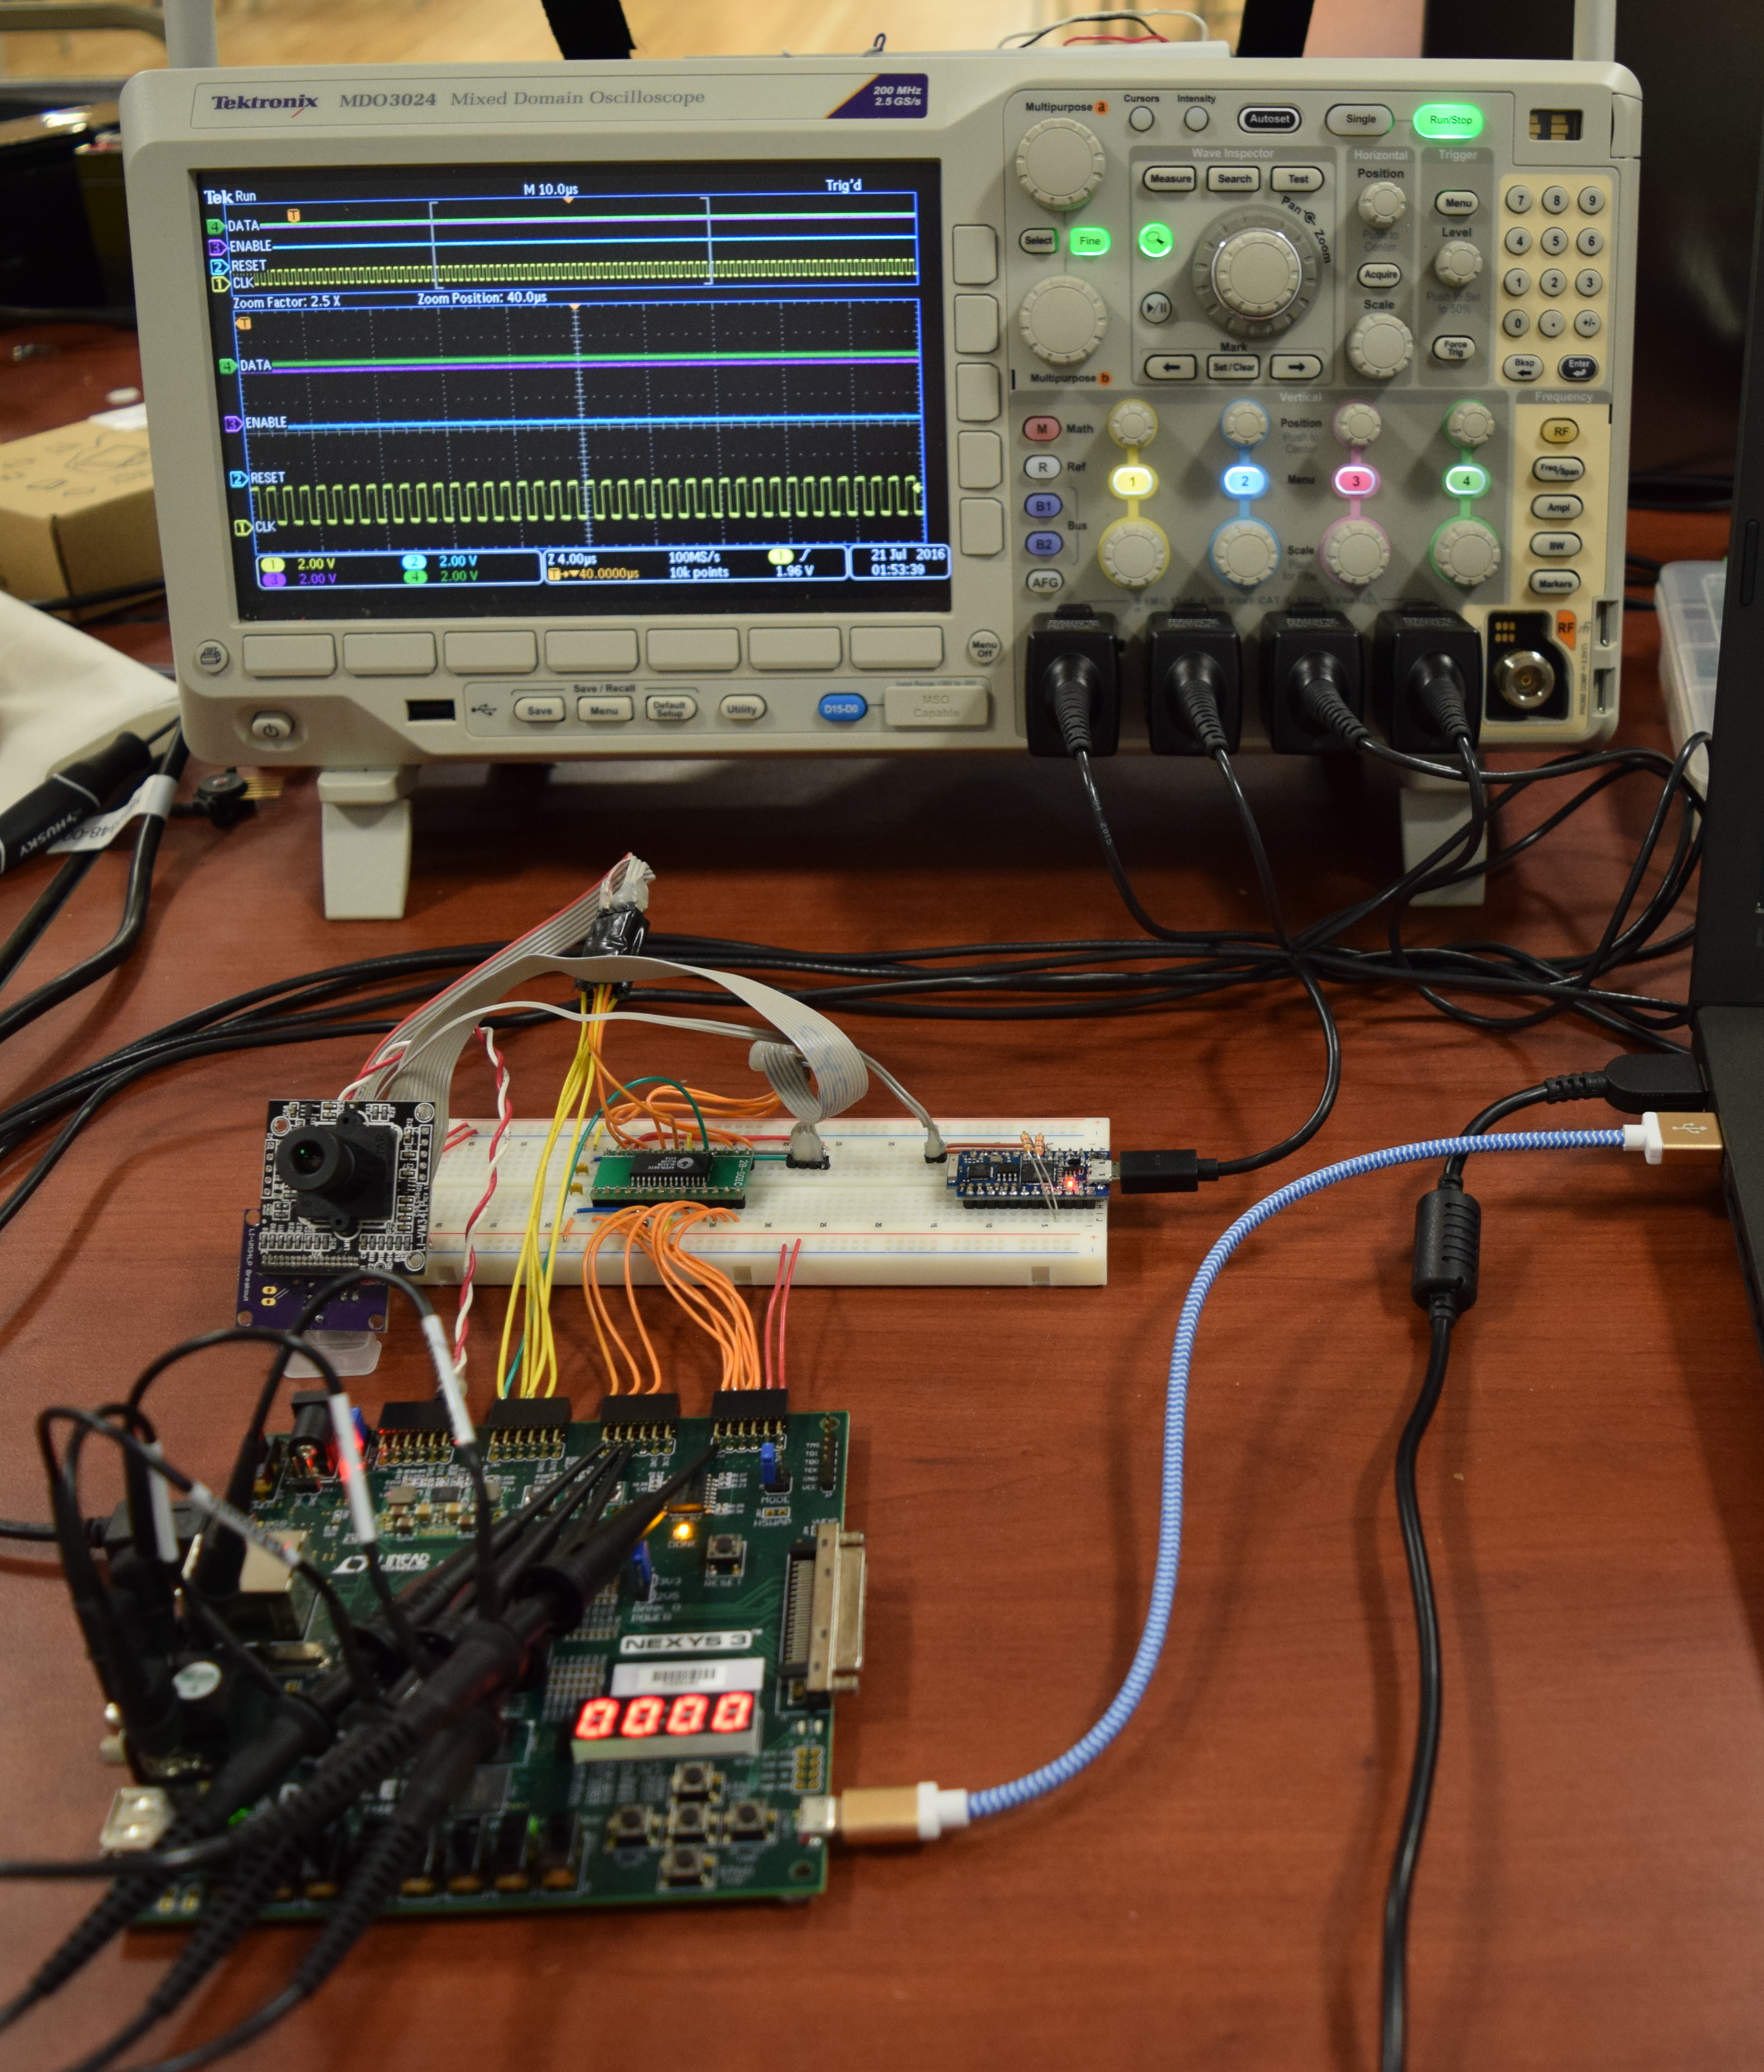
\includegraphics[width=0.5\textwidth]{oScope/camera_fifo/DSC_0010.JPG}}
	\caption{Camera With FIFO and FPGA Control}
	\label{cameraTestSetup}
\end{figure}

\begin{figure}[H]
	\centerline{\includegraphics[width=1.0\textwidth]{oScope/camera_fifo/fifo_rstAndDataTimed.png}}
	\caption{Transferring Line Data from FIFO to FPGA}
	\label{fifoDataOut}
\end{figure}

\subsubsection{Transmitting Images Over UART for Analysis}
The source code found in Appendix item \ref{camTestC} was implemented on a Microblaze MCS in order to transmit camera line data from the FPGA's internal line buffer over UART. An example of the microcontroller's UART output is shown in Figure \ref{PuTTYfifoData}. 
\begin{figure}[H]
	\centerline{\includegraphics[width=0.6\textwidth]{oScope/camera_fifo/PuTTy.png}}
	\caption{Reading FIFO Data}
	\label{PuTTYfifoData}
\end{figure}

\par
After the image was recieved through PuTTy, the \textsc{Matlab} script found in Appendix item \ref{camTestMatlab} was used to parse the corresponding logfile into a greyscale image. An example image created through this process is shown in Figure \ref{notebookImage}. Note that the sub-optimal quality of this image is due to the test setup's wiring. 
\begin{figure}[H]
	\centerline{\includegraphics[width=0.75\textwidth]{oScope/camera_fifo/notebook.png}}
	\caption{Notebook With Grid and Oscilloscope Leads}
	\label{notebookImage}
\end{figure}
